%! TEX root = ../aminhash.tex

\section{Introduction}
Set data (or sparse binary or categorical data) is a staple of data science.
Efficient search and joins of such data is used in document deduplication~\cite{broder1997syntactic}, association rule learning ~\cite{zheng2001real}, and 
for searching genomes and metagenomes in Bioinformatics~\cite{ondov2016mash}.

Quantization is the act of representing data from a large or continuous space by a smaller set of discrete finite values.
Also known as sketching or hashing, this often allows storing very large datasets on a single computer, or on fewer servers than otherwise needed.
At the same time, because the compression and increases data locality, it has become a key component to processing such data efficiently.

%By reducing the space required by data, it not only allows is critical to storing the data at all, it also increases data locality allowing faster search and algorithms working on the quantized data.
%Reducing the space required to store data, it serves a double purpose of increasing data locality for faster search; and of actually allowing the data to be stored in the first place.

MinHash sketches are randomized quantizations of sets (or equivalently $0/1$ vectors).
The idea is to pick $K$ random functions $h_i : U \to [0,1]$ and define the sketch of $X\subseteq U$ to be
\[q(x) = (\argmin_{x\in X}h_1(x), \dots, \argmin_{x\in X}h_K(x)).\]
% TODO: references
After early uses in statistics~\cite{brewer1972selecting} and correlation estimation~\cite{flajolet1985probabilistic}, the term was coined by Broder~\cite{broder1997resemblance, broder1997syntactic} in the context of detecting near-duplicate web pages.
The sketch is known to be near-optimal~\cite{pagh2014min} for estimating set similarity on a given space budget.

A typical scenario is that we want to store some sets $Y_1, \dots$, so we compute the MinHash for each of them, with perhaps $K=30$.
(See \cref{tab:minhash-example} for an example quantized database.)
Now, given a new set, $X$, we quantize it and estimate the similarity with each $Y_i$ by $\|q(X)-q(Y_i)\|_1/K$, which has expectation $\frac{|X\cap Y_i|}{|X\cup Y_i|}$, known as the Jaccard similarity between $X$ and $Y_i$.
Since $q(X)$ only has to be computed once, and each subsequent estimate takes time $O(K)$, rather than $|X \cap Y|$ if we were to compute the Jaccard similarity directly.
Thus, the quantized database can be searched substantially faster than the direct approach.
Sketching can also be combined with space partitions to produce state of the art performing set similarity search~\cite{christiani2018scalable}, but in this paper, we focus on quantization only.

Quantization is also central in state of the art Euclidean nearest neighbour search and Maximum Inner Product Search (MIPS)~\cite{guo2020accelerating}.
In their seminal paper, Jegou et al.~\cite{jegou2010product}
%recognized that compressed representations allow for faster search, even when the data is already dense in $\R^{100}$, say.
%This is mainly due to greater data locality and cache usage.
argued for the application of \emph{asymmetric distance estimation} as a way to improve search accuracy and speed in this context.
Instead of sketching the query and computing the similarity ``in sketch-space'', $\|q(x)-q(y)\|_2$,
one can use the full information of the query and compute $\|x-q(y)\|_2$ reducing the space requirement for equal recall by up to a factor of four.
See~\cref{fig:jegou} for visualization.
%For example, a search engine may store sketches of billions of documents to be searched, but when a query arrives, there is no performance reason to sketch it.

\begin{figure}
   \centering
   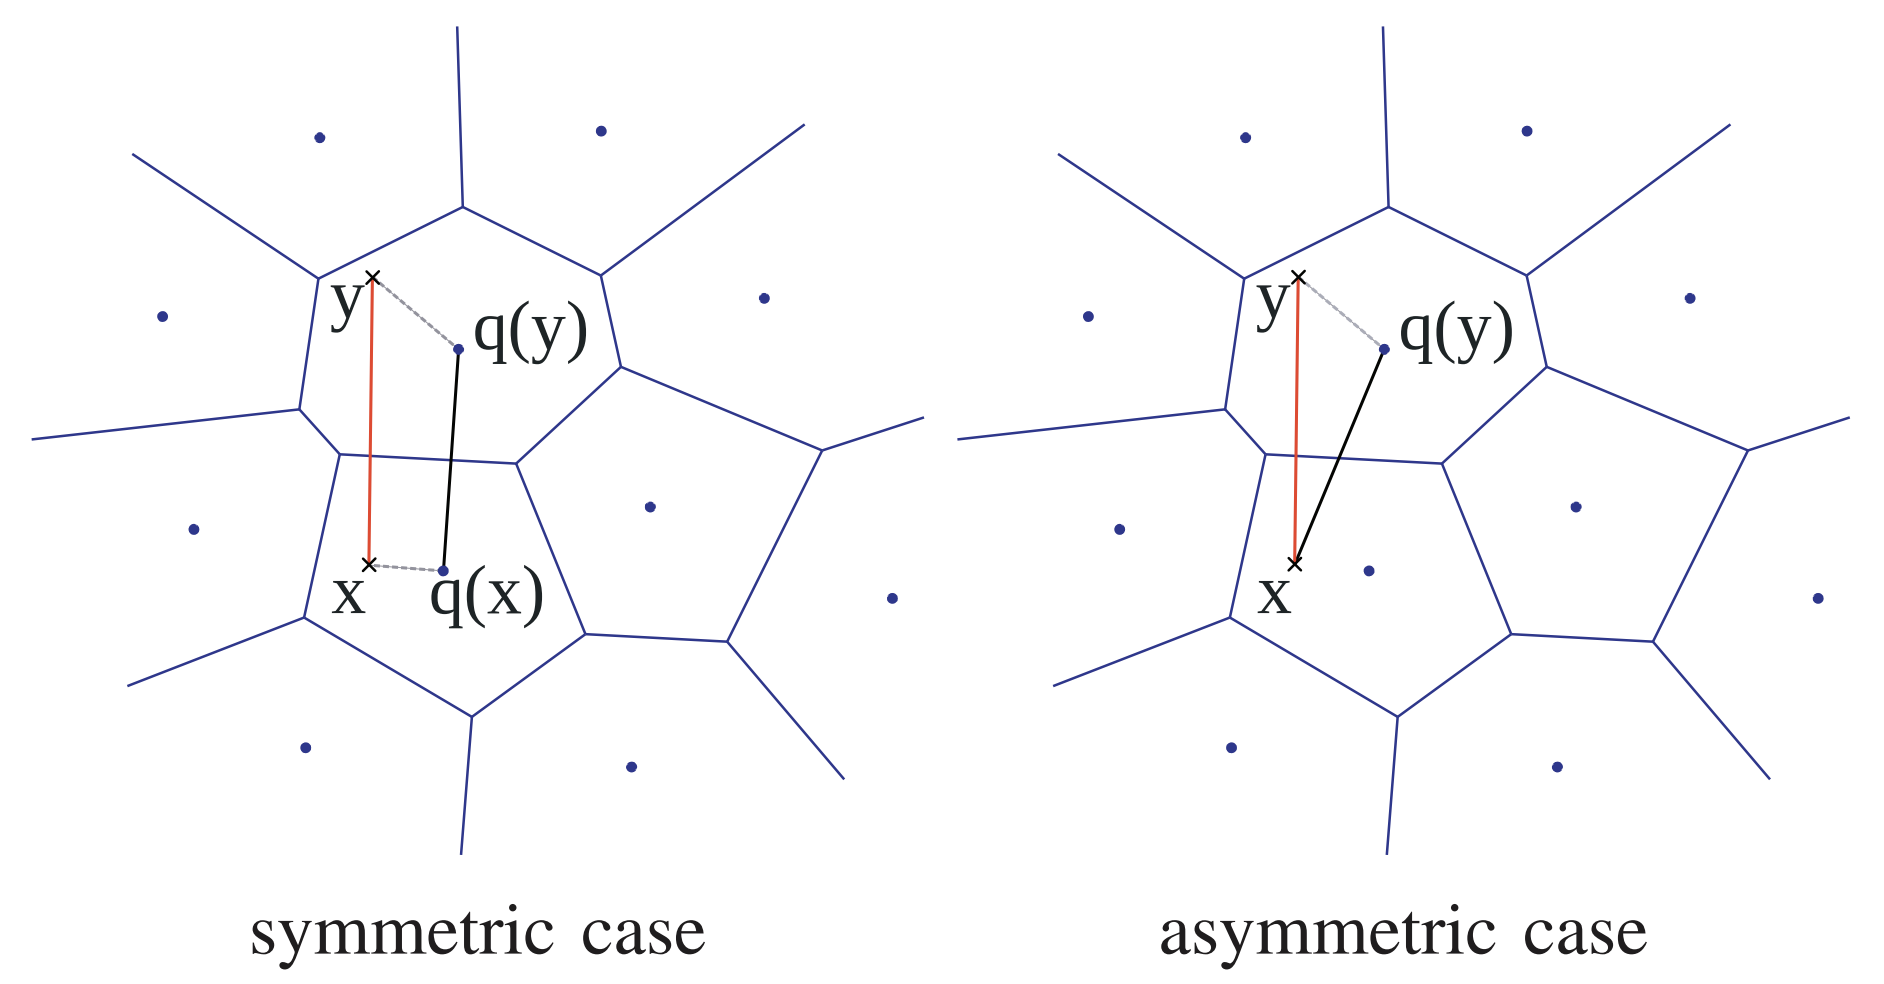
\includegraphics[width=\linewidth]{figures/pq}
\caption{Figure by Jegou et al.~\cite{jegou2010product} illustrating the difference between symmetric and asymmetric estimation, as used in Euclidean Nearest Neighbour Search.
   The distance $q(y)-x$ is a better approximation of $y-x$ than $q(y)-q(x)$.
   In the set setting, when $q$ is MinHash, it is not clear what it would even mean to compute $q(y)-x$?
   %(The voronoi cells are sets that sample to the same minhash value)
}
   \label{fig:jegou}
\end{figure}


While asymmetric estimation is a natural idea for Euclidean distance, it is less clear how it might apply in the context of set search and MinHash quantization.
Somehow we have to compute a similarity value, given $X$ and $q(Y)$ better than $\|q(X)-q(Y)\|_1/K$.
%, since presumably we're throwing information away about $X$ by sketching it.
An indication that this may be possible is the case where the MinHash value of $Y$ is not equal to the MinHash of $X$, but is perhaps equal to the second or third smallest value---that ought to count as evidence towards the sets being similar, even if the classical MinHash sketch would count it as evidence to the opposite.

\subsection{Results}

In this paper, we take a principled approach to this problem.
\begin{enumerate}
   \item We derive an estimator based on maximum likelihood.
      We analyse its variance, which we find to be $28\%$ lower than the classical sketch-space estimator.
      (See figures \ref{fig:mle_variance} and \ref{fig:var}.)
      For small similarities, we reduce the variance by a factor $\frac{|Y|}{|X|+|Y|}$ showing particularly good results when the (known) set $X$ is much larger than the unknown set $Y$.
   \item We investigate relaxations and numerical methods, trading precision for speed of estimation. (See tables \ref{tab:netflix} and \ref{tab:flickr}.)
      A particularly good choice is dubbed the ``Minner Estimator'' since it is based on counting the number of elements in $X$ that hash to a value \emph{smaller than the minimum} hash value of $Y$.
   \item We run experiments on several large set datasets from~\cite{mann2016empirical},
      such as the Netflix dataset originally from \href{https://www.cs.uic.edu/~liub/Netflix-KDD-Cup-2007.html}{KDD-Cup 2007}.
      We show a reduction in the MinHash values needed of up to 30\% for a given recall@10.
\end{enumerate}

While our focus is mainly on applications characterized as ``one-many'', such as search, many applications characterized as ``many-many'' are trivially reduced to $n$ times one-many.
We thus also obtain better performance for important tasks such as duplicate detection and nearest neighbour graph construction.

% TODO: Go over this one more time
A non-goal of the paper is to make the fastest possible implementation of set similarity search.
For this reason, we don't include experiments measuring the runtime of our estimators.
To be competitive in raw running time requires a serious engineering task with papers like~\cite{guo2020accelerating} including 33,812 lines of optimized C and assembly code by many authors.
In \cref{sec:alg} we discuss hardware-level optimizations of this kind.

\subsubsection{Lower $K$ for a given Variance and Recall}

% Rasmus: ``Synes at introen er god. Kunne måske være mere eksplicit om hvad det er du måler. Er plads fx i antal bits eller antal elementer? Hvorfor netop varians?''
Technically, the most difficult part is in the precise variance analysis of the maximum likelihood estimator.
Since our estimators are unbiased, the variance corresponds to the mean squared error when estimating similarity for pairs of sets.
A factor two loss in variance would need to be counterbalanced by a factor two increase in the number of MinHash values, significantly reducing practical performance.
One may ask other questions, such as the necessary $K$ to obtain high probability confidence bounds,
but since we work with independent values, this is mostly trivial.

An important ``downstream'' measure is the recall on real datasets.
This determines how large a $K$ is needed in order to return the true nearest neighbour when scanning a database with estimated similarities.
The exact value depends heavily on the ``difficulty'' of the dataset and varies between 20 and more than 500 for a 90\% recall@10 in our experiments.
In every case our new method is able to obtain a significantly higher recall when given the same information as is available to the classical MinHash estimator.

Other papers have focused on compressing the MinHash sketch itself, a famous algorithm being the~\cite{flajolet2007hyperloglog}.
In general $O(\log\log u + K\log K)$ bits suffice for similarity estimation~\cite{DBLP:reference/algo/Cohen16b}, improving over storing the ranks directly with $\lceil K\log_2 u\rceil$ bits.
Our paper differs by focusing on \emph{reducing $K$}, which can then be combined with those results for even greater compression.
Reducing $K$ also has the benefit of increasing processing speed, something not gained by simply storing the same sketch in less space.
% Why is this more important than things like b-bit minhash?
% Theoretically, this is related to the ``one way communication complexity'' of set similarity.
% In our analysis we focus on minimizing variance (or squared error, since all but one of our estimators are unbiased).
